\section{Motivating Examples}
\label{sec:motiv}

When writing configuration files, the user usually takes already existing files and modifies the, with little knowledge of the system. 
The non-expert user can then easily introduce in errors.
Even worse, the original file may already corrupted and the errors are propagated further. 
Below we show some real worlds examples of the errors commonly found in configuration files.
All these examples are extracted from real-world reports % ~\cite{yin11anempirical, configdataset}.
The deep, domain specific knowledge needed to identify these error manually is strong motivation for a tool such as \app.

\para{Example~1: Ordering Errors.} When configuring PHP to run with the Apache HTTP Server the user writes, among others, the following lines:\\
 \texttt{
 \hspace*{3em}extension = mysql.so\\
 \hspace*{3em}...\\
 \hspace*{3em}extension = recode.so}\\
This file caused the Apache server to fail to start due to a segmentation fault error.
When using PHP in Apache, the extension ``mysql.so'' depends on ``recode.so'' and the relative ordering of two of them is crucial. 
\app would inform the user that ``recode.so'' should appear before ``mysql.so'', and return the error:\\
 \texttt{
ORDERING ERROR: Expected "extension"recode.so"\\
   BEFORE "extension""mysql.so"
  }

\para{Example~2: Entry Missing Errors.} If the user wants to use OpenLDAP to enable her directory access
protocol, she needs to use the password policy overlay. This is usually
done through the following entries in the OpenLDAP configuration file:\\
\texttt{
 \hspace*{3em}include schema/ppolicy.schema\\
 \hspace*{3em}overlay ppolicy\\}
When using the password policy overlay in OpenLDAP, we have to first include the related schema.
Leaving out the ``include'' statement will cause this LDAP server fail to work:\\
Running \app on such a misconfiguration file would return:\\
\texttt{
MISSING KEYWORD ERROR: Expected "overlay""ppolicy"\\ 
in the same file as: "include""schema/ppolicy.schema"}

\para{Example~3: Type Errors.} If the user tries to install MySQL, she first needs to initiate the path for the log information generated by MySQL. 
A user may put the following code in the MySQL configuration file:\\
\texttt{
 \hspace*{3em}general\_log = /var/log/mysql/mysql.log\\}
However, the entry ``general\_log'' should be an integer, not a string.
 In MySQL, there is another entry named ``general\_log\_file'' which is used to specify the log path.  
After \app analyzes this configuration file, it correctly identifies the error:\\
\texttt{
TYPE ERROR: Expected a Int with P=1.0 for "general\_log[mysqld]"
}

\para{Example~4: Value Correlation Errors.} When configuring PHP on MySQL, the user may write the following lines of entries in both the PHP and MySQL configuration files:\\
\texttt{
 \hspace*{3em}mysql's config\\
 \hspace*{3em}max\_connections = 300\\
 \hspace*{3em}...\\
 \hspace*{3em}php's config\\
 \hspace*{3em}mysql.max\_persistent = 400\\}
This could cause MySQL to abort with the error information: ``too many connections''.
In this case, the ``mysql.max\_persistent'' in PHP should be no larger than the ``max\_connections'' in MySQL configuration file.
Another rule we have implemented is learning inequality relations between integers.
Running \app on this combined configuration file would return:
\texttt{
INTEGER RELATION ERROR: \\
Expected "max\_connections">="mysql.max\_persistent"}




\com{
\begin{figure}[t] \centering
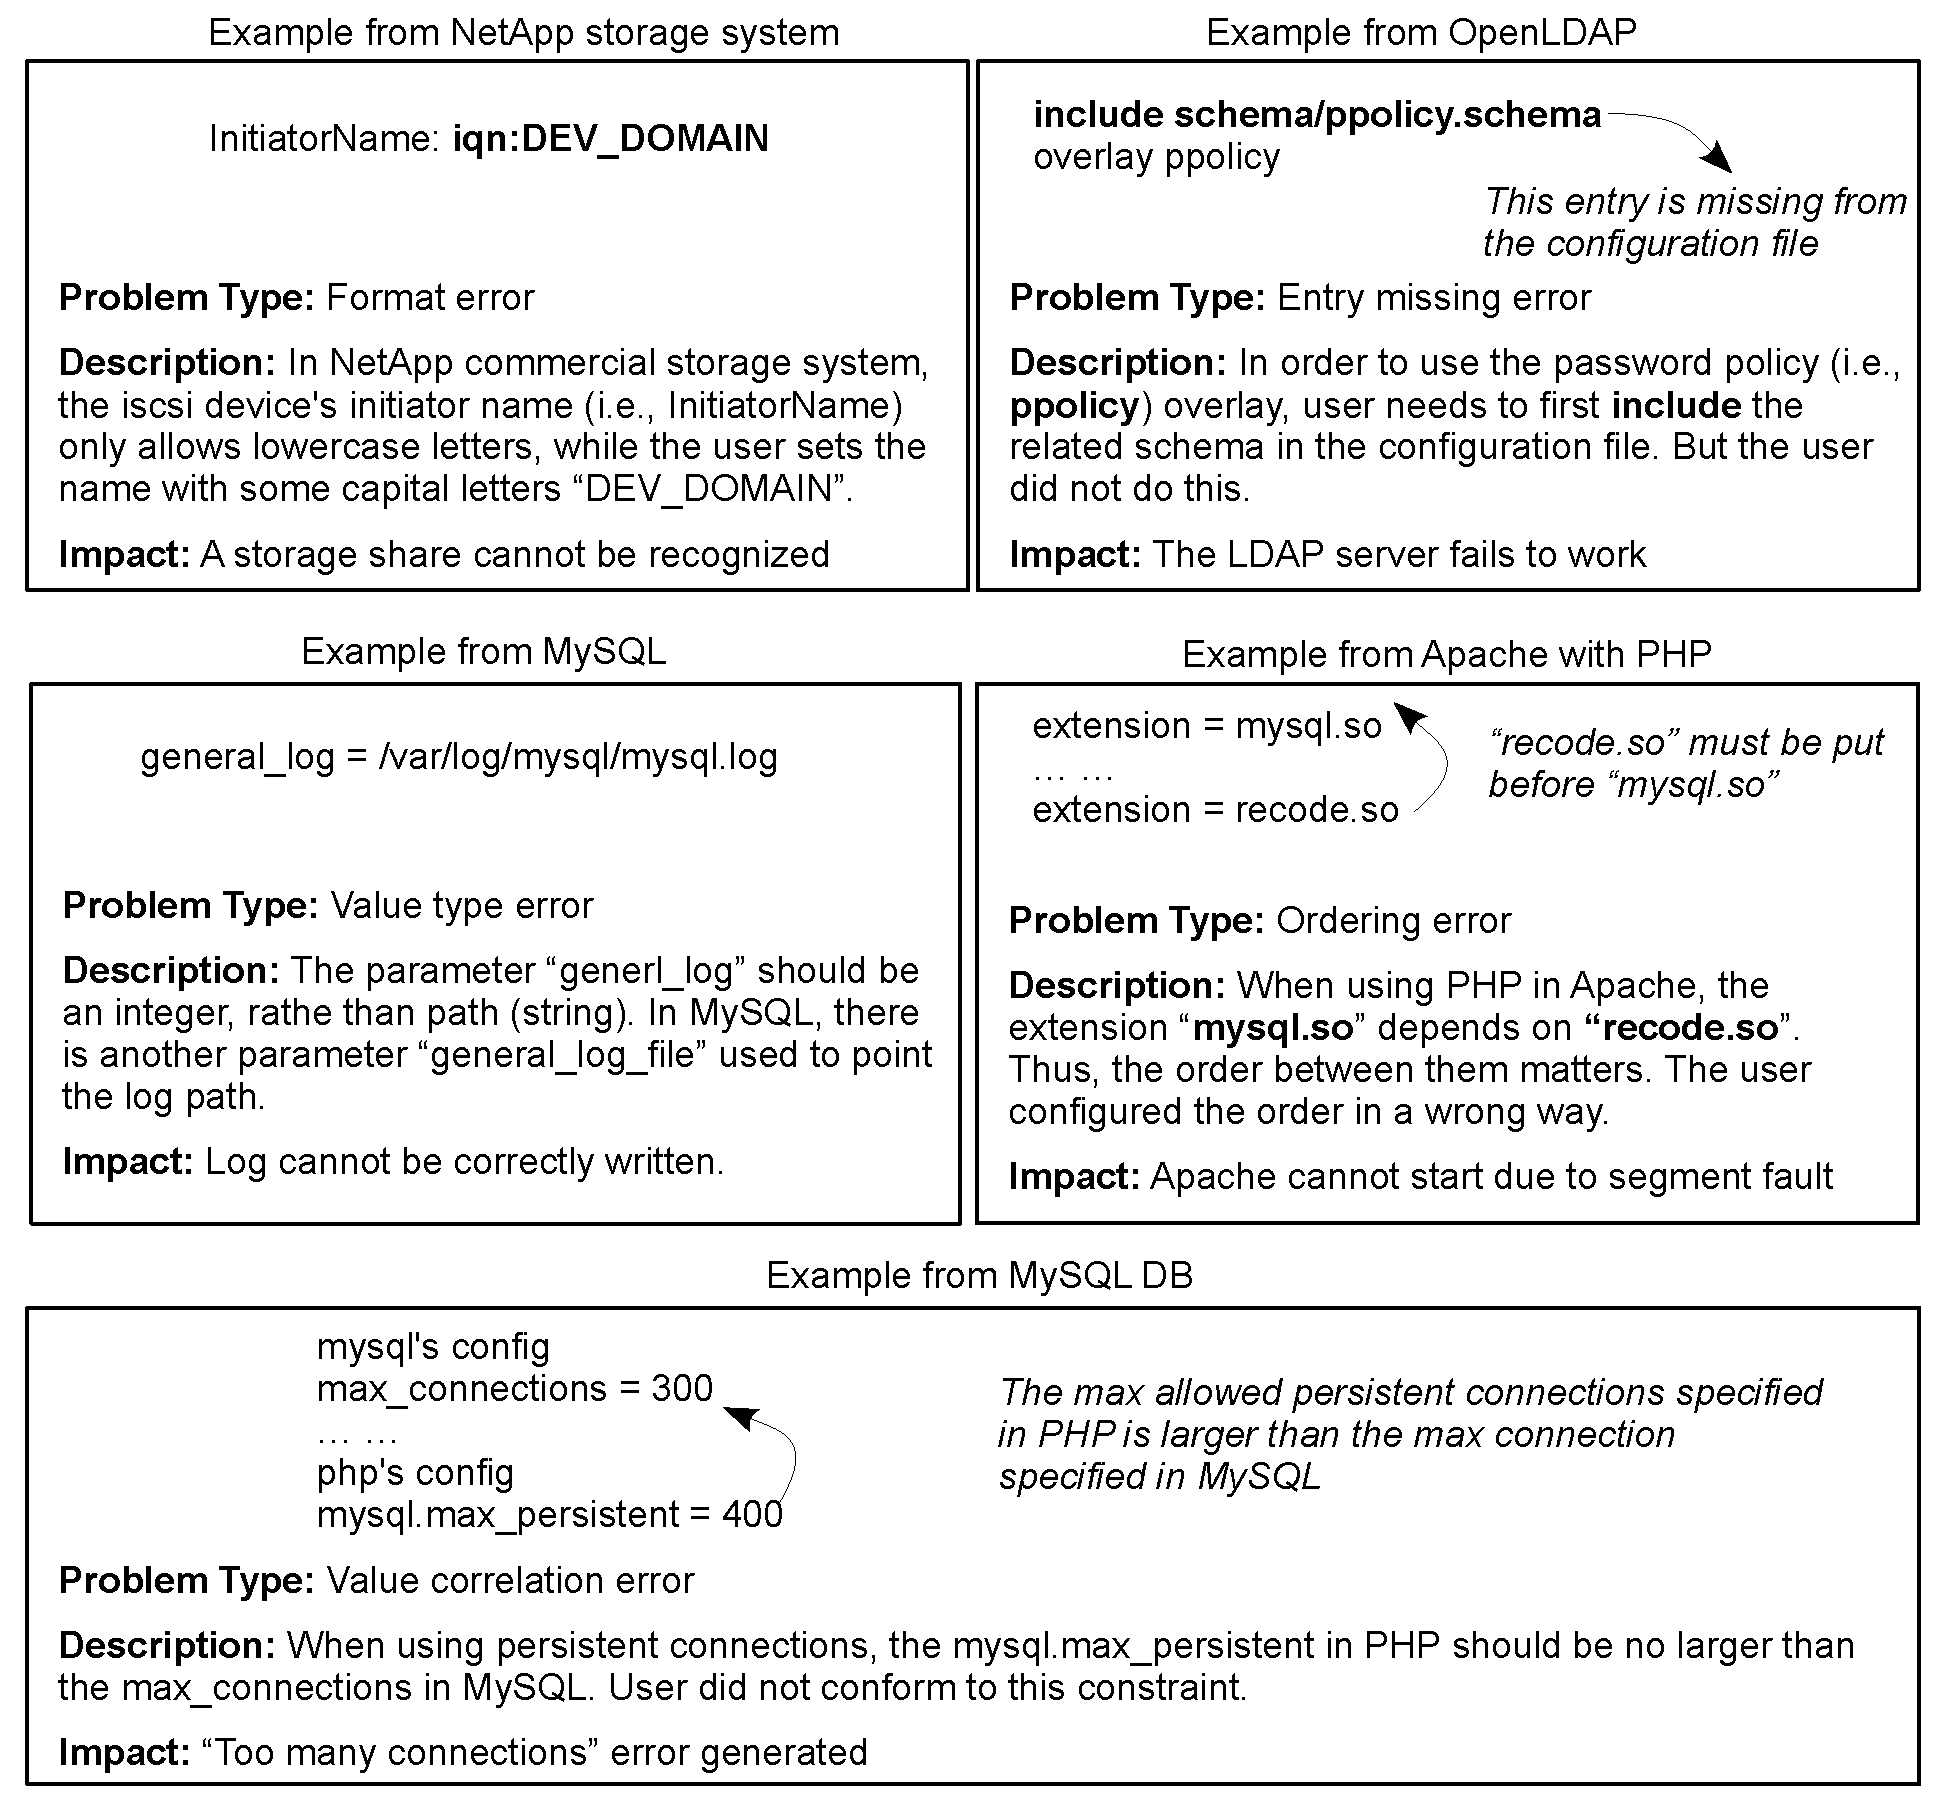
\includegraphics[width=0.98\textwidth]{figs/example}
\caption{Motivating examples. Our target configuration errors are
  classified into five groups. The five examples here correspond to
  these groups, respectively.}
\label{fig-example}
\end{figure}

Fig.~\ref{fig-example} presents misconfiguration examples in real-world
that we aim to address. All the examples are extracted from
misconfiguration issues reported in real-world efforts%
~\cite{yin11anempirical, configdataset}.
We classify our target configuration errors
into five groups: 1) format error; 2) entry missing error; 3) value type
error; and 4) ordering error
The examples in Fig.~\ref{fig-example} correspond to the above four
groups, respectively.

} 
